\documentclass{beamer}
\usepackage[T1]{fontenc}
\usepackage[utf8]{inputenc}
\usepackage[frenchb]{babel}
\usepackage{graphicx}
\usepackage{subfig}
\usepackage{colortbl}
\usepackage{tikz}
\usepackage{bm}
\usepackage{listings}

%listins
\lstset{
language=C++,
frame=single,
keywordstyle=\color{magenta}\bfseries,
commentstyle=\color{green}\itshape,
stringstyle=\color{blue},
showstringspaces=true,
showspaces=false,
breaklines=true,
breakatwhitespace=true,
tabsize=2}


\graphicspath{{Images/}}

\usetheme{Hannover}

\beamertemplatenavigationsymbolsempty

\AtBeginSection[]
  {
     \begin{frame}<beamer>
     \frametitle{Plan}
     \tableofcontents[currentsection]
     \end{frame}
  }

\definecolor{bleufonce}{rgb}{0.1,0.1,0.8}
\definecolor{grisbleu}{rgb}{0.8,0.8,0.9}
\definecolor{rougefonce}{rgb}{0.8,0.1,0.1}
\definecolor{grisrouge}{rgb}{0.9,0.8,0.8}
\definecolor{vertfonce}{rgb}{0.1,0.8,0.1}
\definecolor{grisvert}{rgb}{0.8,0.9,0.8}
\definecolor{bleuunistra}{RGB}{15,80,150}
\setbeamercolor{palette quaternary}{fg=white,bg=bleuunistra}
\setbeamercolor{titlelike}{parent=palette quaternary}

\setbeamertemplate{blocks}[rounded][shadow=true] 
\setbeamercolor{block title}{bg=bleufonce,fg=white}
\setbeamercolor{block body}{bg=grisbleu}
\setbeamercolor{block title alerted}{bg=rougefonce,fg=white}
\setbeamercolor{block body alerted}{bg=grisrouge}
\setbeamercolor{block title example}{bg=vertfonce,fg=white}
\setbeamercolor{block body example}{bg=grisvert}

\newcommand{\grad}{{\nabla}}
\newcommand{\laplace}{{\Delta}}
\newcommand{\rot}{{\nabla\times}}
\newcommand{\rott}{{\nabla^2\times}}
\renewcommand{\div}{{\nabla\cdot}}
\newcommand{\restr}{{\big\rvert_{\partial\Omega}}}
\newcommand{\taille}{0.4}
\newcommand{\taillem}{0.5}
\newcommand{\tailleg}{0.7}
\newcommand{\Ctaille}{0.5}
\newcommand{\Ctaillem}{0.6}
\newcommand{\Ctailleg}{0.8}

\title[Stage]{Parallélisation d'un code de calcul aérodynamique instationnaire et validation par comparaison avec des données existantes.}
\subtitle{Plastic Omnium, M2 CSMI}

\author{Romain HILD}
\institute{Université de Strasbourg}

\begin{document}

\begin{frame}

\includegraphics[scale=0.2]{uds.jpg}
\includegraphics[scale=0.15]{po.jpg}
\titlepage
\end{frame}

\begin{frame}{Plastic Omnium}
\begin{itemize}
\item Société fondée en 1946 par Pierre Burelle.
\item Transforme et commercialise des matières plastiques.
\item Scindée en deux entités :
\begin{itemize}
\item Plastic Omnium Environnement
\item Plastic Omnium Automobile
\end{itemize}
\item Objectifs :
\begin{itemize}
\item réduire le poids
\item augmenter l'aérodynamisme
\item équiper les véhicules hybrides et électriques
\end{itemize}
\end{itemize}
\centering
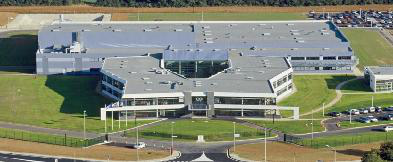
\includegraphics[scale=0.5]{sigma}
\end{frame}

\section{Problème}
\begin{frame}{Problème}
\begin{block}{On cherche $(\mathbf{v},p)$ solution de :}
\begin{equation}
\label{depart}
\left\{\begin{aligned}
&\frac{\partial \mathbf{v}}{\partial t} + (\rot  \mathbf{v})\times \mathbf{v} + \grad q + \frac{1}{Re}\rott  \mathbf{v}-\mathbf{f} = 0\\
&\div \mathbf{v} = 0\\
&\mathbf{v}\big\rvert_{t=0} = \mathbf{v}_0\\
&\mathbf{v}\cdot \mathbf{n}\restr = \alpha_0\\
&(\rot  \mathbf{v})\cdot \mathbf{n}\restr = \alpha_1\\
&(\rott  \mathbf{v})\cdot \mathbf{n}\restr = \alpha_2
\end{aligned}\right.
\end{equation}
où $q = \frac{|\mathbf{v}|^2}{2}+p$.
\end{block}
Conditions aux bords :
\begin{itemize}
\item condition d'ordre 2
\item composante normale nulle
\item composante tangentielle libre
\end{itemize}
\end{frame}

\begin{frame}{Problème}
\begin{block}{Séparation des variables}
On veut exprimer la solution sous la forme
\[ \sum_i c_i(t) \mathbf{g}_i(x,y,z) \]
\begin{itemize}
\item les coefficients $c_i$ portent la dimension temporelle.
\item les fonctions de base $(\mathbf{g}_i)$ portent la dimension spatiale.
\end{itemize}
\end{block}
Utilisation des travaux de P. Penel :
\begin{itemize}
\item $D^1(\Omega) = \{\mathbf{v} \in [H^1(\Omega)]^3\; |\; \div\mathbf{v}=0,\nabla^k\times \mathbf{v}\cdot \mathbf{n} = 0, k=0,1 \}$
\item engendré par les fonctions propres de l'opérateur rotationnel
\item relèvement des conditions aux limites,
\end{itemize}
\end{frame}

\begin{frame}
\centering
\begin{tikzpicture}
\node[draw,fill=green!50] (alpha0) at (0,10) {$\alpha_0$};
\node[draw,fill=gray!50,align=center] (pbpsi0) at (0,8.5) {Problème\\ Poisson} ;
\node[draw,fill=blue!50] (gradpsi0) at (0,7) {$\grad\psi^0$} ;
\node[draw,fill=green!50] (alpha1) at (2.5,10) {$\alpha_1$};
\node[draw,fill=gray!50,align=center] (pbcurlb) at (2.5,8.5) {Problème\\ mixte} ;
\node[draw,fill=blue!50] (curlb) at (2.5,7) {$(\rot\mathbf{b},\grad\psi^1)$} ;
\node[draw,fill=gray!50] (pba) at (1.25,6) {$\mathbf{a}=\grad\psi^0+\rot\mathbf{b}$};
\node[draw,fill=blue!50] (a) at (1.25,5) {$\mathbf{a}$} ;
\node[draw=red,align=center,fill=gray!50] (pbeigen) at (7.5,8.5) {Problème\\ aux valeurs\\ propres} ;
\node[draw,fill=yellow!50] (lambdagi) at (7.5, 7) {$(\Lambda_i,\mathbf{g_i})$} ;
\node[draw,fill=green!50] (alpha2) at (4.25,7) {$\alpha_2$};
\node[draw,fill=green!50] (f) at (5,7) {$\mathbf{f}$};
\node[draw,fill=green!50] (c0) at (6,7) {$c_i(0)$};
\node[draw=red,align=center,fill=gray!50] (pbc) at (6,5) {Problème spectral};
\node[draw,fill=blue!50] (u) at (5,3.75) {$\mathbf{u}$} ;
\node[draw,fill=gray!50] (pbv) at (3,3) {$\mathbf{v}=\mathbf{a}+\mathbf{u}$} ;
\node[draw,fill=red!50] (v) at (3,2) {$(\mathbf{v},p)$} ;

\draw[->,>=latex] (alpha0) -- (pbpsi0); \draw[->,>=latex] (pbpsi0) -- (gradpsi0); \draw[->,>=latex] (alpha1) -- (pbcurlb); \draw[->,>=latex] (pbcurlb) -- (curlb); \draw[->,>=latex] (gradpsi0) -- (pba); \draw[->,>=latex] (curlb) -- (pba); \draw[->,>=latex] (pba) -- (a); \draw[->,>=latex] (pbeigen) -- (lambdagi); \draw[->,>=latex] (a) -- (pbc); \draw[->,>=latex] (alpha2) -- (pbc); \draw[->,>=latex] (f) -- (pbc); \draw[->,>=latex] (c0) -- (pbc); \draw[->,>=latex] (lambdagi) -- (pbc); \draw[->,>=latex] (pbc) -- (u); \draw[->,>=latex] (u) -- (pbv); \draw[->,>=latex] (a) -- (pbv); \draw[->,>=latex] (pbv) -- (v);
\end{tikzpicture}
\end{frame}

\section{Fonctions propres}
\begin{frame}{$\mathbf{u}=\sum_{i=1}^\infty c_i\mathbf{g}_i$}
\begin{block}{Propriétés des modes propres}
\begin{itemize}
\item les fonctions propres de $\rot\star$ sont aussi celles de $\rott\star$.
\item les valeurs propres de $\rot\star$ sont les racines carrées de celles de $\rott\star$.
\item pour ne pas avoir de multiplicité > 1, on ne garde que les positives : $\lambda_i=\sqrt{\Lambda_i}$
\item le signe est porté par le coefficient $c_k$.
\end{itemize}
\end{block}
\begin{block}{Trouver $(\mathbf{g},\lambda)\in D^1\times \mathbb{R}$ tel que}
\[\left\{\begin{aligned}
&\rott  \mathbf{g}_i = \lambda_i^2 \mathbf{g}_i\\
&(\div \mathbf{g}_i = 0)\\
&\mathbf{g}_i\cdot \mathbf{n}\restr = 0\\
&\rot \mathbf{g}_i\cdot \mathbf{n}\restr = 0\\
&(\rott  \mathbf{g}_i\cdot \mathbf{n}\restr = 0)
\end{aligned}\right.\]
\end{block}
\end{frame}

\begin{frame}{Résultats}
\begin{figure}[H]
	\makebox[\textwidth][c]{
		\subfloat[mode 0]{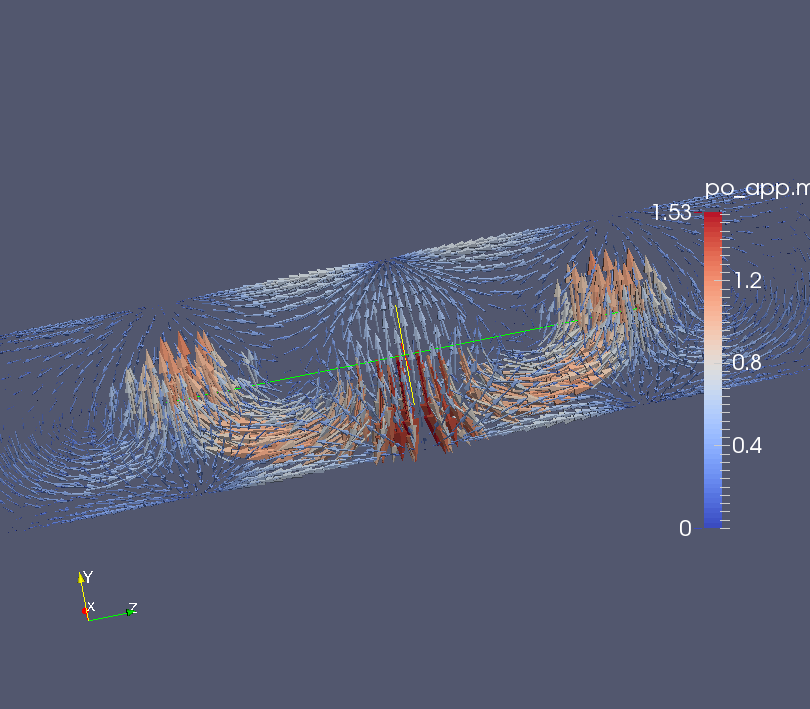
\includegraphics[scale=0.15,trim=0mm 10mm 0mm 40mm,clip]{curl-grad-1e3-mode0}}\ 
		\subfloat[mode 45]{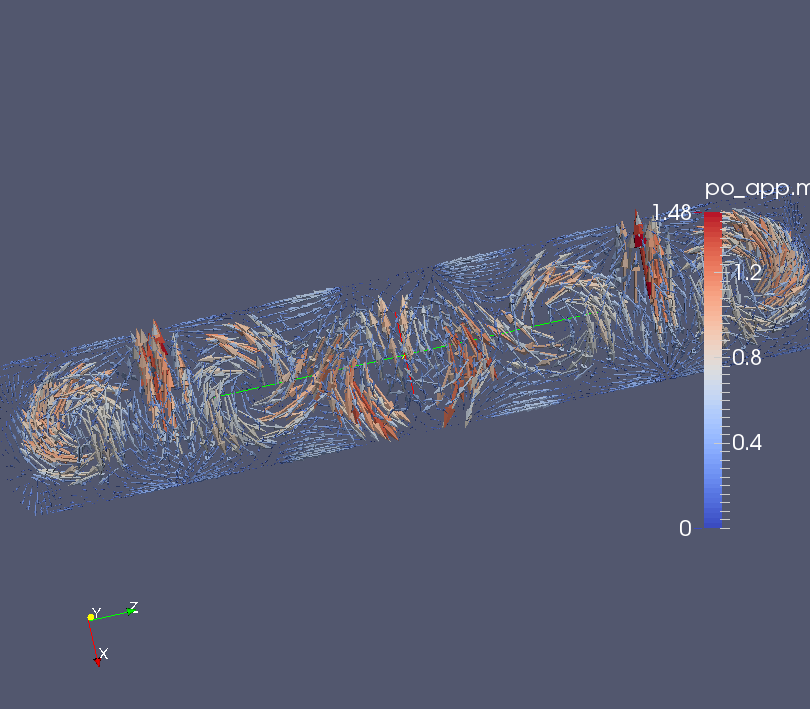
\includegraphics[scale=0.15,trim=0mm 10mm 0mm 40mm,clip]{curl-grad-1e3-mode45}}
	}
	\makebox[\textwidth][c]{
		\subfloat[tps/nombre de modes]{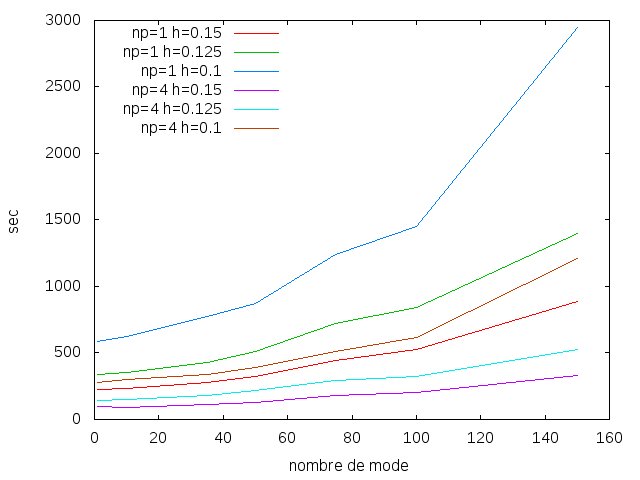
\includegraphics[scale=0.3]{timeM}}\ 
		\subfloat[tps/taille maillage]{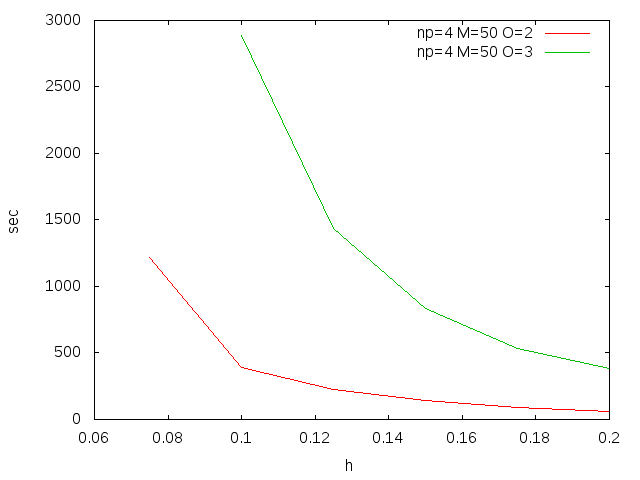
\includegraphics[scale=0.3]{timeH}}
	}
\end{figure}

\end{frame}

\section{Relèvement}
\begin{frame}{Relèvement}
\label{psi0}
\begin{block}{Décomposition de $\mathbf{a}$}
\begin{center}
\begin{tabular}{c|ccccc}
& $\mathbf{a}$ & = & $\grad\psi^0$ & + & $\rot \mathbf{b}$ \\ \hline
$\div\star$ & 0 & & $\laplace\psi^0$ & & 0\\ \hline
$\star\cdot \mathbf{n}\restr$ & $\alpha_0$ & & $\alpha_0$ & & 0\\ \hline
$\rot\star\cdot \mathbf{n}\restr$ & $\alpha_1$ & & 0 & & $\alpha_1$
\end{tabular}
\end{center}
\end{block}
2 choix pour le relèvement de $\alpha_0$ par $\grad\psi^0$ :
\begin{itemize}
\item Laplacien dans $H^1$
\item Problème mixte dans $H(\mathrm{div})$
\end{itemize}
2 choix pour le relèvement de $\alpha_1$ par $\rot\mathbf{b}$ :
\begin{itemize}
\item Problème mixte dans $H(\mathrm{rot})$
\item utilisation de la base $(\mathbf{g}_i)$ dans $D^1$
\end{itemize}
\end{frame}

\begin{frame}{Résultats}
\centering
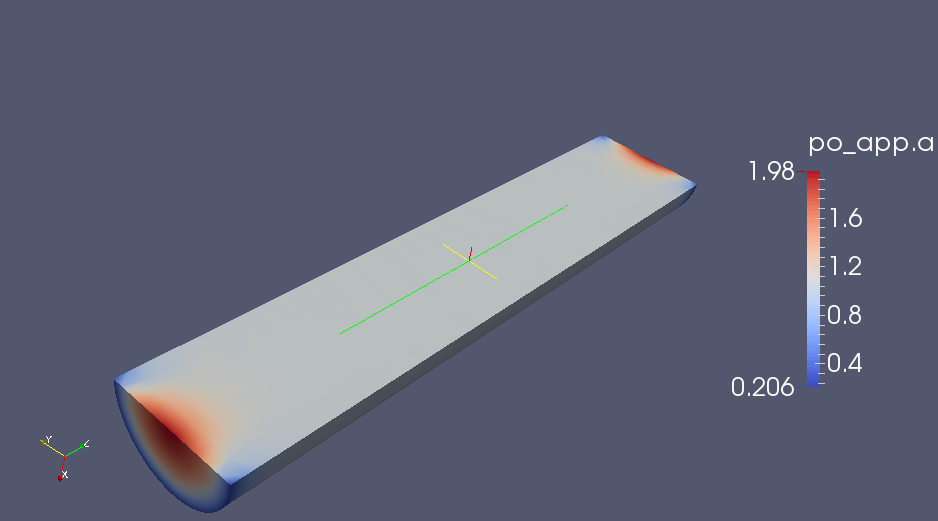
\includegraphics[scale=0.2]{psi0-clip}
\begin{figure}[H]
	\makebox[\textwidth][c]{
		\subfloat[entrée]{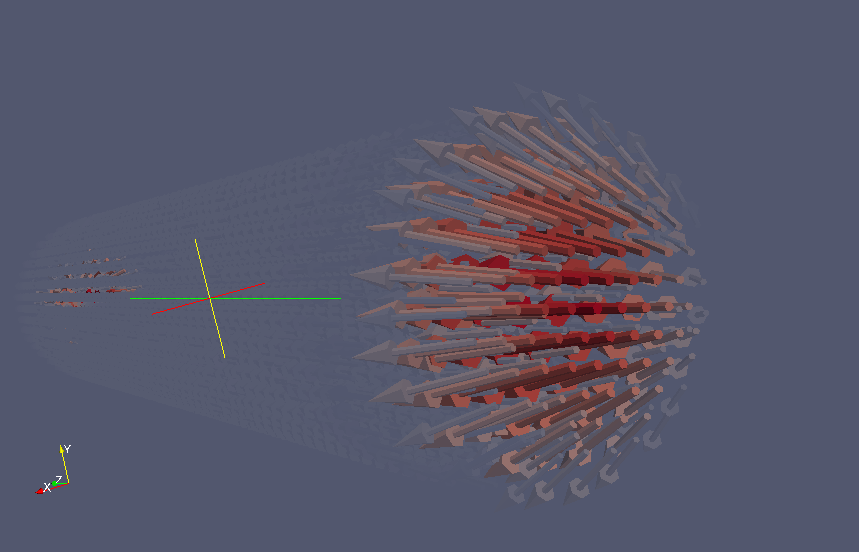
\includegraphics[scale=0.15]{aIn}}\ 
		\subfloat[sortie]{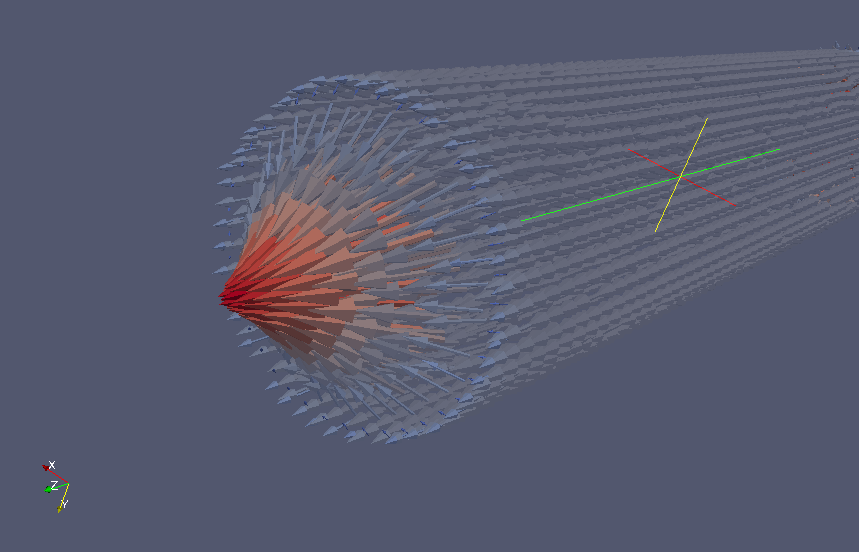
\includegraphics[scale=0.15]{aOut}}
	}
\end{figure}
\end{frame}

\section{Problème spectral}
\begin{frame}{Problème spectral}
En utilisant $\mathbf{v}=\mathbf{u}+\mathbf{a}$ dans (\ref{depart}), on obtient :
\begin{align*}
\frac{\partial \mathbf{u}}{\partial t} &+ (\rot \mathbf{u})\times \mathbf{u} + (\rot \mathbf{u})\times \mathbf{a} + \left(\rot \mathbf{a}\right)\times \mathbf{u} \\
&+ \grad\pi_\mathbf{a} + \frac{1}{Re}\rott \mathbf{u} - \mathbf{f_a} = 0
\end{align*}
où : $\pi_a=\frac{|\mathbf{u}+\mathbf{a}|^2}{2}$ et $\mathbf{f_a}=\mathbf{f}-\frac{\partial \mathbf{a}}{\partial t}-(\rot\mathbf{a})\times\mathbf{a}$.
\begin{block}{Trouver $\mathbf{u}\in D^1$ tel que $\forall \bm{\varphi}=\bm{\varphi}_0+\grad\phi\in D^1$ :}
\begin{align*}
\int_\Omega \frac{\partial \mathbf{u}}{\partial t}\cdot \bm{\varphi} &+ \int_\Omega ((\rot \mathbf{u})\times \mathbf{u})\cdot \bm{\varphi} + \int_\Omega ((\rot \mathbf{u})\times \mathbf{a})\cdot\bm{\varphi} \\
&+ \int_\Omega ((\rot \mathbf{a})\times \mathbf{u})\cdot\bm{\varphi} + \frac{1}{Re}\int_\Omega (\rot \mathbf{u})\cdot(\rot\bm{\varphi}) \\
&-\frac{1}{Re}\int_{\partial\Omega} \alpha_2\phi = \int_\Omega \mathbf{f_a}\cdot\bm{\varphi}
\end{align*}
\end{block}
\end{frame}

\begin{frame}{Discrétisation}
En utilisant $\mathbf{u}_M=\sum_{i=1}^M c_i\mathbf{g}_i$ et en notant :
\begin{align*}
R_{ijk} &= \lambda_i\int_\Omega(\mathbf{g_i}\times \mathbf{g_j})\cdot\mathbf{g_k} & R_{iak} &= \lambda_i\int_\Omega(\mathbf{g_i}\times \mathbf{a})\cdot\mathbf{g_k}\\
R_{raij} &= \int_\Omega((\rot\mathbf{a})\times \mathbf{g_i})\cdot\mathbf{g_k} & R_{hk} &= \int_\Omega\mathbf{f_a}\cdot\mathbf{g_k}\\
R_{pk} &= \int_{\partial\Omega} \alpha_2\phi_k
\end{align*}
On a le problème suivant :
\begin{block}{Trouver $(c_i)_{i=1,\dots,M}$ tel que $\forall k=1,\dots,M$ :}
\[ \frac{\partial c_k}{\partial t} + \frac{1}{Re}c_k\lambda_k^2 + \sum_{i,j=1}^Mc_ic_jR_{ijk} + \sum_{i=1}^Mc_i\left(R_{iak} + R_{raij}\right) = R_{hk} + \frac{1}{Re}R_{pk} \]
\end{block}
\end{frame}

\begin{frame}{Résultats}
\begin{figure}[H]
	\makebox[\textwidth][c]{
      \subfloat{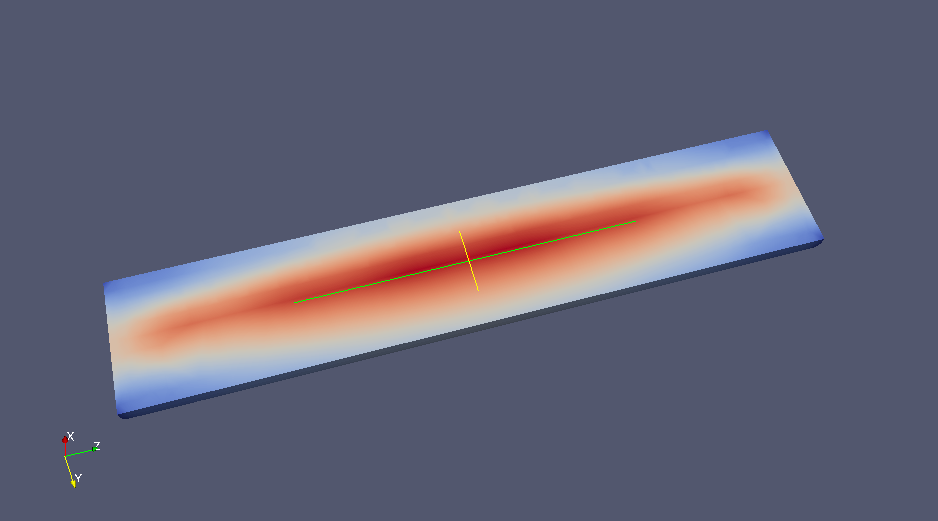
\includegraphics[scale=0.15,trim=0mm 20mm 0mm 20mm,clip]{v100modes}}\ 
		\subfloat{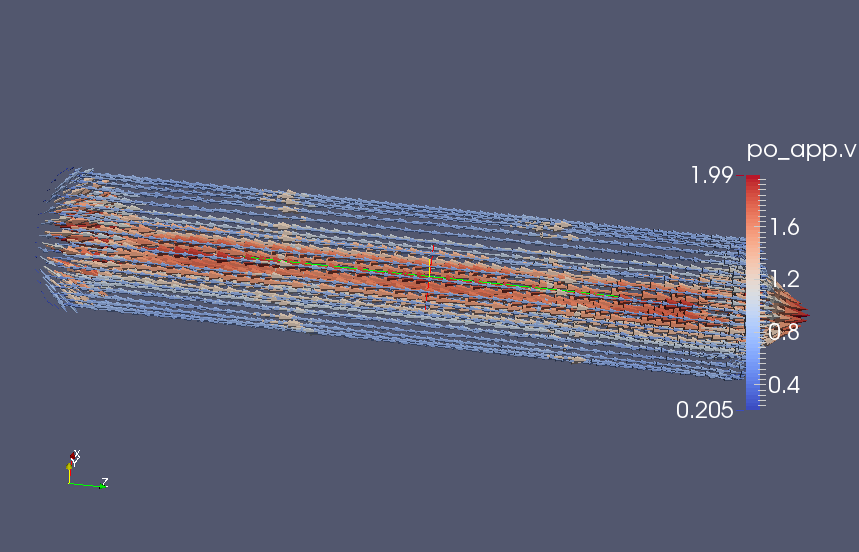
\includegraphics[scale=0.15,trim=0mm 20mm 0mm 30mm,clip]{vGradPression32-32}}
	}
\caption{M = 50}
\end{figure}
\begin{figure}[H]
	\makebox[\textwidth][c]{
      \subfloat[M=10]{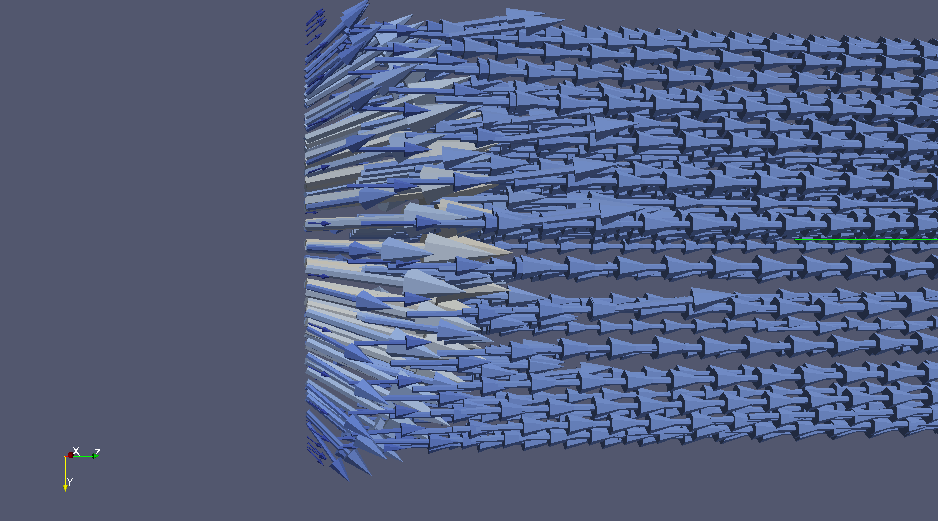
\includegraphics[scale=0.25,trim=100mm 20mm 100mm 20mm,clip]{vIn10}}\ 
		\subfloat[M=100]{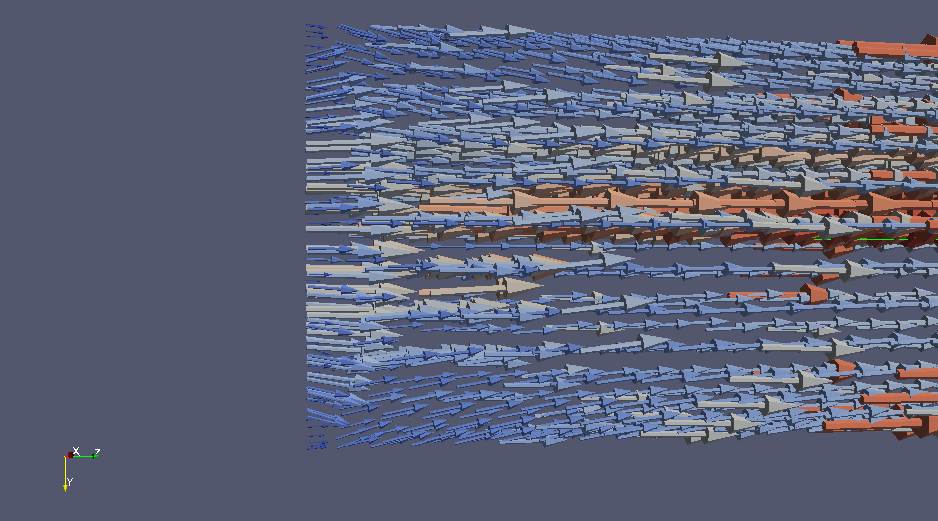
\includegraphics[scale=0.25,trim=100mm 20mm 100mm 20mm,clip]{vIn100}}
	}
\end{figure}
\end{frame}

\section{Conclusion}
\begin{frame}
\begin{figure}
\centering
\begin{tikzpicture}[scale=0.4] 
\node[draw,scale=\taille,fill=green!50] (a0) at (0.75,2) {$\alpha_0$} ;
\node[draw,scale=\taille,fill=gray!50] (pbpsi0lp) at (-0.5,-2)
{$\begin{aligned}
-\laplace\psi^0&=0\\
\grad\psi^0\cdot \mathbf{n} &= \alpha_0
\end{aligned}$} ;
\node[draw,scale=\taille,fill=blue!50] (psi0) at (-0.5,-3.5) {$\psi^0$} ;
\node[draw,scale=\taille,fill=gray!50] (pbgradpsi0) at (-0.5,-4.75) {$w=\grad\psi^0$} ;
\node[draw,scale=\taille,fill=gray!50] (pbpsi0div) at (2,-2)
{$\begin{aligned}
\mathbf{w}&=\grad\psi^0\\
\div\mathbf{w}&=0\\
\mathbf{w}\cdot \mathbf{n} &= \alpha_0
\end{aligned}$} ;
\node[draw,scale=\taille,fill=blue!50] (gradpsi0) at (0.75,-8.75) {$\grad\psi^0$} ;
\node (psi0Im) at (-3.5,-8.75) {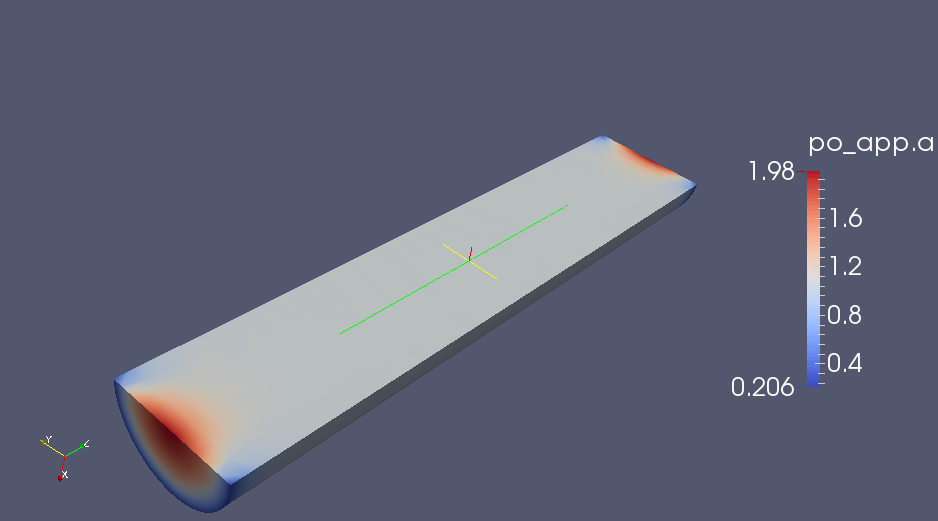
\includegraphics[scale=0.1,angle=90,trim=35mm 0mm 80mm 0mm,clip]{psi0-clip}} ;

\node[draw,scale=\taille,fill=green!50] (a1) at (5.5,2) {$\alpha_1$} ;
\node[draw,scale=\taille,fill=gray!50] (pbbcurl) at (4,-5)
{$\begin{aligned}
\rott \mathbf{b} &= \grad\psi^1\\
\div \mathbf{b} &=0\\
\mathbf{b}\cdot \mathbf{n} &= 0\\
\rot \mathbf{b}\cdot \mathbf{n} &= 0\\
\grad \psi^1\cdot \mathbf{n} &= \alpha_1
\end{aligned}$} ;
\node[draw,scale=\taille,fill=gray!50] (pbpsi1lp) at (7,-2)
{$\begin{aligned}
-\laplace\psi^1&=0\\
\grad\psi^1\cdot \mathbf{n} &= \alpha_1
\end{aligned}$} ;
\node[draw,scale=\taille,fill=blue!50] (psi1) at (7,-3.5) {$\psi^1$} ;
\node[draw,scale=\taille,fill=gray!50] (pbgradpsi1) at (7,-4.75) {$w=\grad\psi^1$} ;
\node[draw,scale=\taille,fill=gray!50] (pbpsi1div) at (9.5,-2)
{$\begin{aligned}
\mathbf{w}&=\grad\psi^1\\
\div \mathbf{w}&=0\\
\mathbf{w}\cdot \mathbf{n} &= \alpha_1
\end{aligned}$} ;
\node[draw,scale=\taille,fill=blue!50] (gradpsi1) at (8.25,-6) {$\grad\psi^1$} ;
\node[draw,scale=\taille,fill=gray!50
] (pbb) at (8,-7.5) 
{$
d_k\lambda_k^2 = (\grad\psi^1,\mathbf{g_k}) - \langle\alpha_1,\psi_k\rangle
$} ;
\node[draw,scale=\taille,fill=blue!50] (b) at (5.5,-8.75) {$\rot \mathbf{b}$} ;

\node[draw,scale=\taille,fill=gray!50] (pbeigen) at (13.5,2)
{$\begin{aligned}
\rott \mathbf{g_i} = \Lambda_i\mathbf{g_i}\\
\div\mathbf{g_i} = 0\\
\mathbf{g_i}\cdot \mathbf{n}\restr = 0\\
\rot \mathbf{g_i}\cdot \mathbf{n}\restr = 0\\
(\rott \mathbf{g_i}\cdot \mathbf{n}\restr = 0)
\end{aligned}$} ;
\node[draw,scale=\taille,fill=yellow!50] (lambdagi) at (13.5,-0.5) {$(\Lambda_i,\mathbf{g_i})$} ;
\node[draw,scale=\taille,fill=gray!50] (pbgi0) at (13.5,-3)
{$\begin{aligned}
\grad(\div \mathbf{g_i^0})-\laplace \mathbf{g_i^0} &= \Lambda_i\mathbf{g_i}\\
\mathbf{g_i^0} &= 0
\end{aligned}$} ;
\node[draw,scale=\taille,fill=yellow!50] (gi0) at (13.5,-4.5) {$\mathbf{g_i^0}$} ;
\node[draw,scale=\taille,fill=gray!50] (pbpsi) at (13,-6)
{$\begin{aligned}
-\laplace\psi_i = \div \mathbf{g_i^0}\\
\grad\psi_i\cdot \mathbf{n}\restr = 0
\end{aligned}$} ;
\node[draw,scale=\taille,fill=yellow!50] (psi) at (12.5,-7.5) {$\psi_i$} ;

\node[draw,scale=\taille,fill=gray!50] (pba) at (2,-10.5) {$\mathbf{a} = \rot \mathbf{b} + \grad\psi^0$} ;
\node[draw,scale=\taillem,fill=blue!50] (a) at (2,-12) {$\mathbf{a}$} ;

\node[draw,scale=\taille,fill=green!50] (f) at (7,-9) {$f$} ;
\node[draw,scale=\taille,fill=green!50] (a2) at (8,-9) {$\alpha_2$} ;
\node[draw,scale=\taille,fill=green!50] (ck0) at (9,-9) {$c_k^0$} ;
\node[draw,scale=\taille,fill=gray!50] (pbs) at (9,-12)
{$\begin{aligned}
\frac{\partial c_k}{\partial t} &+ \frac{1}{Re}c_k\lambda_k^2 + \sum_i\sum_j c_i c_j R_{ijk}\\
&+ \sum_i c_i R_{iak} + \sum_i c_i R_{raik} = R_{fk} + \frac{1}{Re}R_{pk}
\end{aligned}
$} ;
\node[draw,scale=\taillem,fill=blue!50] (u) at (9,-14.5) {$\mathbf{u}$} ;
\node (uIm) at (15,-15) {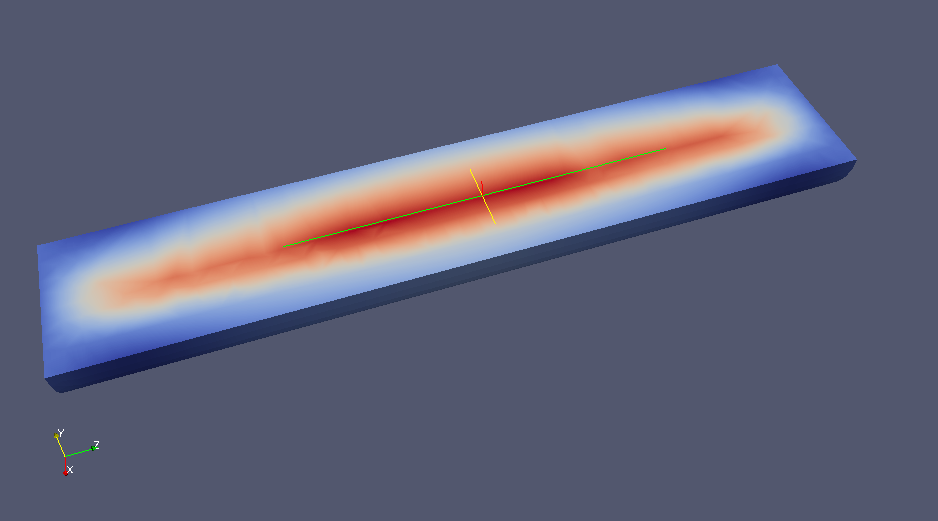
\includegraphics[scale=0.1,trim=0mm 40mm 20mm 15mm,clip]{u-clip}} ;
\node[draw,scale=\tailleg,fill=red!50] (v) at (5,-16) {$(\mathbf{v},p)$} ;
\node (vIm) at (-1,-16) {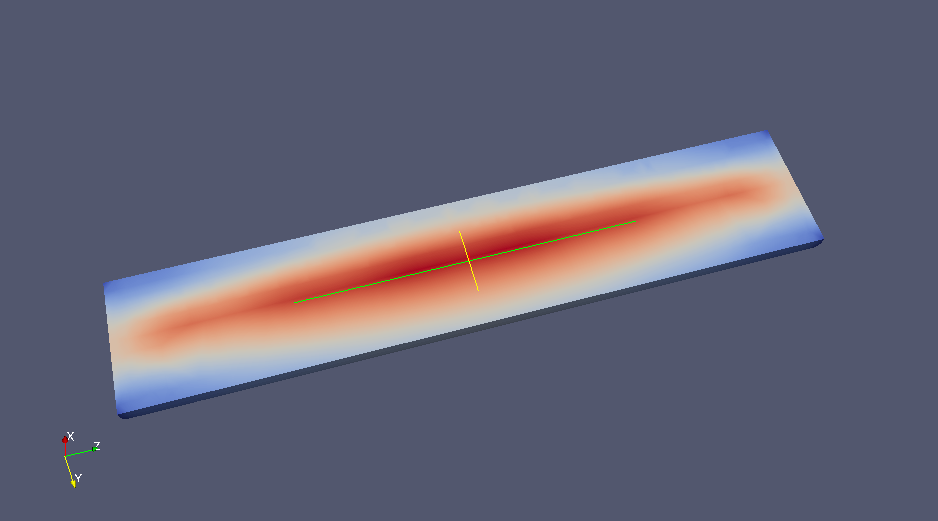
\includegraphics[scale=0.1,trim=0mm 30mm 20mm 30mm,clip]{v100modes}} ;

\draw (a0) -- (0.75,0);
\draw[->,>=latex] (gradpsi0) -- (pba) ;
\draw[->,>=latex,purple] (0.75,0) -| (pbpsi0lp) ;
\draw[->,>=latex,purple] (pbpsi0lp) -- (psi0) ;
\draw[->,>=latex,purple] (psi0) -- (pbgradpsi0) ;
\draw[->,>=latex,purple] (pbgradpsi0) -- (gradpsi0) ;
\draw[->,>=latex,green] (0.75,0) -| (pbpsi0div) ;
\draw[->,>=latex,green] (pbpsi0div) -- (gradpsi0) ;
\draw[<->,>=latex] (gradpsi0) -- (psi0Im) ;

\draw (a1) -- (5.5,1);
\draw[->,>=latex,magenta] (5.5,1) -| (pbbcurl) ;
\draw[->,>=latex,magenta] (pbbcurl) -- (b) ;
\draw[cyan] (5.5,1) -| (8.25,0);
\draw[->,>=latex,orange] (8.25,0) -| (pbpsi1div);
\draw[->,>=latex,red] (8.25,0) -| (pbpsi1lp);
\draw[->,>=latex,red] (pbpsi1lp) -- (psi1);
\draw[->,>=latex,red] (psi1) -- (pbgradpsi1);
\draw[->,>=latex,red] (pbgradpsi1) -- (gradpsi1);
\draw[->,>=latex,orange] (pbpsi1div) -- (gradpsi1);
\draw[->,>=latex,cyan] (gradpsi1) -- (pbb);
\draw[->,>=latex,cyan] (psi) -- (pbb);
\draw[->,>=latex,cyan] (lambdagi) to[out=180,in=40] (pbb.15);
\draw[->,>=latex,cyan] (pbb) -- (b);
\draw[->,>=latex] (b) -- (pba);

\draw[->,>=latex] (pba) -- (a);
\draw[->,>=latex] (pbeigen) -- (lambdagi);
\draw[->,>=latex] (lambdagi) -- (pbgi0);
\draw[->,>=latex] (pbgi0) -- (gi0);
\draw[->,>=latex] (gi0) -- (pbpsi);
\draw[->,>=latex] (pbpsi) -- (psi);
\draw[->,>=latex] (a) -- (pbs);
\draw[->,>=latex] (f) -- (pbs);
\draw[->,>=latex] (a2) -- (pbs);
\draw[->,>=latex] (ck0) -- (pbs);
\draw[->,>=latex] (lambdagi) to[out=-10,in=20] (pbs.east);
\draw[->,>=latex] (psi) -- (pbs);
\draw[->,>=latex] (pbs) -- (u);
\draw[<->,>=latex] (u) -- (uIm) ;
\draw[->,>=latex] (u) -- (v);
\draw[->,>=latex] (a) -- (v);
\draw[<->,>=latex] (v) -- (vIm) ;
\end{tikzpicture}
\end{figure}
\end{frame}

\begin{frame}{Temps de calcul}
\centering
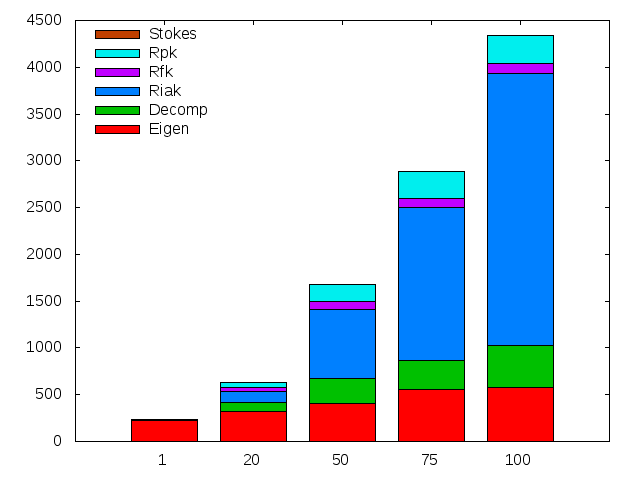
\includegraphics[scale=0.6]{histo}
\end{frame}

\begin{frame}{Perspectives}
\begin{itemize}
\item Tests sur une machine plus puissante
\begin{itemize}
\item Plus de modes
\item Taille de mailles plus petites
\end{itemize}
\item Utilisation des éléments conformes
\begin{itemize}
\item Nedelec
\item $D^1$
\end{itemize}
\item Relèvement de $\alpha_2$
\begin{itemize}
\item Décomposition des modes inutiles
\end{itemize}
\item Géométries industrielles
\end{itemize}
\end{frame}

\begin{frame}
\begin{center}
Merci de votre attention !
\end{center}
\end{frame}


\end{document}
